% !TeX root = ../main.tex

\chapter{补充材料}


\section{补充章节}

补充内容。
\subsection{压缩感知理论数学表述}
压缩感知用于图像重建分为三个主要模块:
\begin{enumerate}
  \item 观测矩阵的设计
  \item 信号的稀疏化表示
  \item 图像信息从稀疏代码的重构
\end{enumerate}

\begin{figure}[ht]
  \centering
  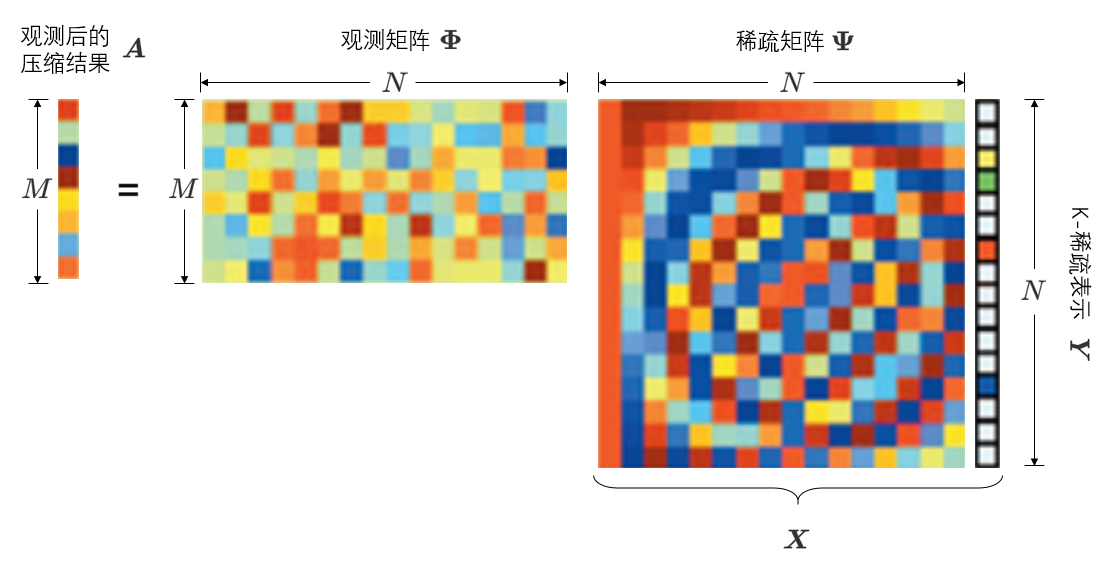
\includegraphics[width=\textwidth]{cs_principle_image.png}
  \caption{观测值,原始值和稀疏代码}

\end{figure}
第一步观测矩阵的设计数学表达如下
\begin{equation}
  \label{eq:9}
  y = \Phi x
\end{equation}

其中$y \in R^{M \times 1}$为压缩感知的观测值,是对真实信号的一种采样,$x \in R^{N \times 1}$为原始图像信号。这里对x进行拉平处理,将一般情况下的二维图像信号拉平为一维信号便于数学处理。$\Phi \in R^{M \times N}$是测量矩阵,其作用是对原始图像信号进行采样。在此公式中,压缩比例为$\frac{M}{N}$。且为了保证且为了突破传统的奈奎斯特采样定律,需要选择合适的测量矩阵使得 $M \ll N$。在这个阶段,压缩本身是无损的。而之所以能够突破这个采样定律,是因为这个定律是建立在周期性的连续信号等间距采样上的,且没有对原始信号进行其他域上的变换。对于图像这样非周期性的数据,奈奎斯特采样是不足以充分描述和应用的。用非等间距采样例如随即亚采样往往能更好的体现出图像各个部分信息类型、密度不均匀的性质。更进一步地,为了从远小于未知解的方程个数中还原出原图像,还应该保证RIP(Restricted Isometry Property)条件,使得信号在K稀疏的条件下可以从M个参数中得到最优解。2005年Tao等人\cite{Decoding_by_linear_programming}提出了保证最优解唯一的等效RIP条件,此证明作为压缩感知原始信号还原的可行性和质量的保证。也证明,独立同分布的随机高斯采样矩阵能够作为普适的采样矩阵。下图是不同的采样矩阵的图例,

\begin{figure}[ht]
  \centering
  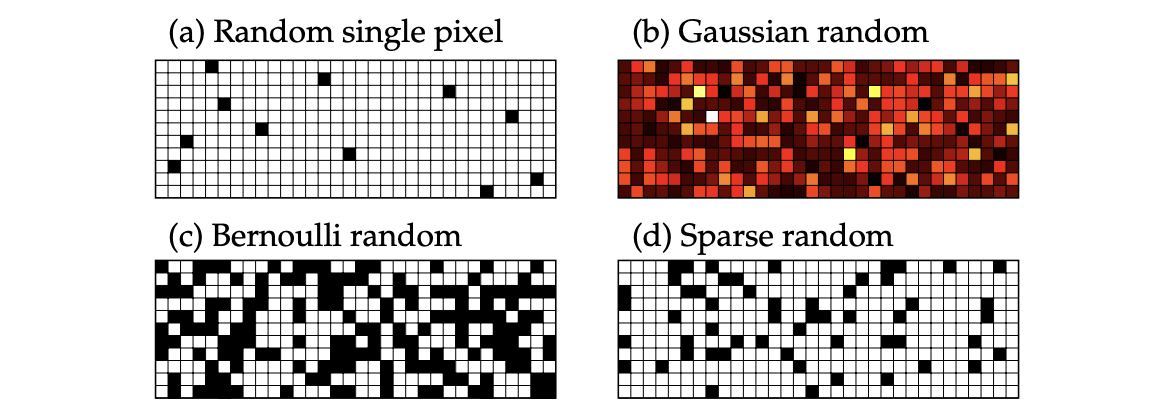
\includegraphics[width=\textwidth]{random_matrix.png}
  \label{fig:random_sample_matrix}
  \caption{不同的采样矩阵}
\end{figure}

2006年Emmanuel等人\cite{Emmanuel2006Stable}证明了在已知信号稀疏性的情况下,可能凭借较采样定理所规定更少的采样数重建原信号,这一理论也是压缩感知的基石,对RIP的必要性做了进一步的阐释。2007年Bananiuk等人\cite{2008A}简化了满足RIP条件的矩阵验证,在该技术从理论走向实践的过程中贡献。


第二步信号的稀疏化表示的数学表达如下
\begin{equation}
  \label{eq:10}
  x = \Psi a
\end{equation}

其中x为公式\ref{eq:9}中的原始图像信号。在真实世界的普通摄像设备对常规物体拍摄的二维图像中,图像在空间上具备较强的相关性。且图像的像素排列表示并不满足稀疏条件,不存在大量值为0的元素,因此在这一步中通过设计合适的稀疏矩阵$\Psi \in R^{N \times N}$
将x变化为转换域上的信号$a \in R^{N \times 1}$。如果a向量中有K个非零元素,则称a向量为K稀疏向量。
此时联立\ref{eq:9}与\ref{eq:10}可得到

\begin{equation}
  \label{eq:14}
  y = \Phi x = \Phi \Psi a = \Theta a
\end{equation}
其中$\Theta = \Phi \Psi, \Theta \in R^{M \times N}$,称其为传感矩阵。此时我们可以详细的列出RIP条件。由于多篇文章定义形式不一,这里采用\cite{The_restricted_isometry_property_and_its_implications_for_compressed_sensing}中定义的RIP条件。

\begin{equation}
  \label{eq:13}
  (1-\delta_k) \Vert a \Vert_2^2 \leq \Vert \Theta a \Vert_2^2 \leq (1+\delta_k) \Vert a \Vert_2^2
\end{equation}

即每一个整数$k \in \left[1,N\right]$,定义矩阵$\Theta$的等距系数$\delta_{k}$为在所有k稀疏向量a情况下,都满足\ref{eq:13}公式的最小值。
从能量的角度考虑,$\Vert \Theta a \Vert_2^2 = \Vert y\Vert_2^2$,即为观测信号的能量,而根据公式\ref{eq:10}将原始信号分解成稀疏代码的矩阵$\Psi$是正交变换,根据Parseval变换定理正交变换不改变信号能量。所以通过引入参数$\delta_k$使得前后能量的差值满足一定的范围,即观测矩阵和标准正交矩阵的差别不能够超出一定范围。对应到向量上,RIP条件是保证k稀疏向量在分解过程之中对应不为0的分量的能量不存在剧烈的增幅或衰减。如果允许$\delta_k = 0$,则$\Vert a \Vert_2^2 = \Vert y\Vert_2^2$,二者能量完全相等,证明观测矩阵本身亦是正交变换,而按照公式\ref{eq:13}定义,$\delta_k \in (0,1)$,所以这证明$\Phi$不可能是正交矩阵,保证了$M < N$这个压缩的前提。

在2008年Bananiuk等人\cite{Compressive_sensing_[Lecture_Notes]}解决了RIP问题易于定义不便寻找的问题,提出了RIP的等价定义,即$\Phi$与$\Psi$之间彼此不相关,相关性定义如下:

\begin{equation}
  \label{eq:11}
  \mu(\phi, \psi) = \sqrt{n} \cdot \mathop{\max}_{1 \leq k,j \leq n} |<\phi_k,\psi_j>| \Rightarrow \mu(\phi, \psi) \in \left[ 1,\sqrt{n}  \right]
\end{equation}

其中$\mu(\phi, \psi)$越接近于1,则越不相关。将\ref{eq:14}转变成优化问题如下

\begin{equation}
  \label{eq:12}
  \min \Vert a \Vert_0 \quad \text{s.t.} \quad y = \Phi x = \Phi \Psi a
\end{equation}

第三步图像信息从稀疏代码的重构即是将优化所得结果a代回\ref{eq:10}则可求出原始信号x。但是考虑到$\Phi \in R^{M \times N}$ 且  $M \ll N$,那么上述优化问题是一个NP难问题,无法直接求解。需要将公式进行改造以转换为凸优化问题或者采用贪婪算法进行近似求解。2008年Emmanual等人\cite{The_restricted_isometry_property_and_its_implications_for_compressed_sensing}证明了当$\delta_{2k} < 1$时可以保证零范数问题有唯一的稀疏解,而当$\delta_{2s}<\sqrt2-1$时则可以保证0范数和1范数等价。零范数求解为NP-hard问题,在此前提下将其转化为1范数求最优化问题,由于此时问题被转换为凸优化问题,所以可以保证其局部最优解即为全局最优解。

对公式\ref{eq:12}添加不同的约束项会得到不同的目标函数。

\begin{figure}[ht]
  \centering
  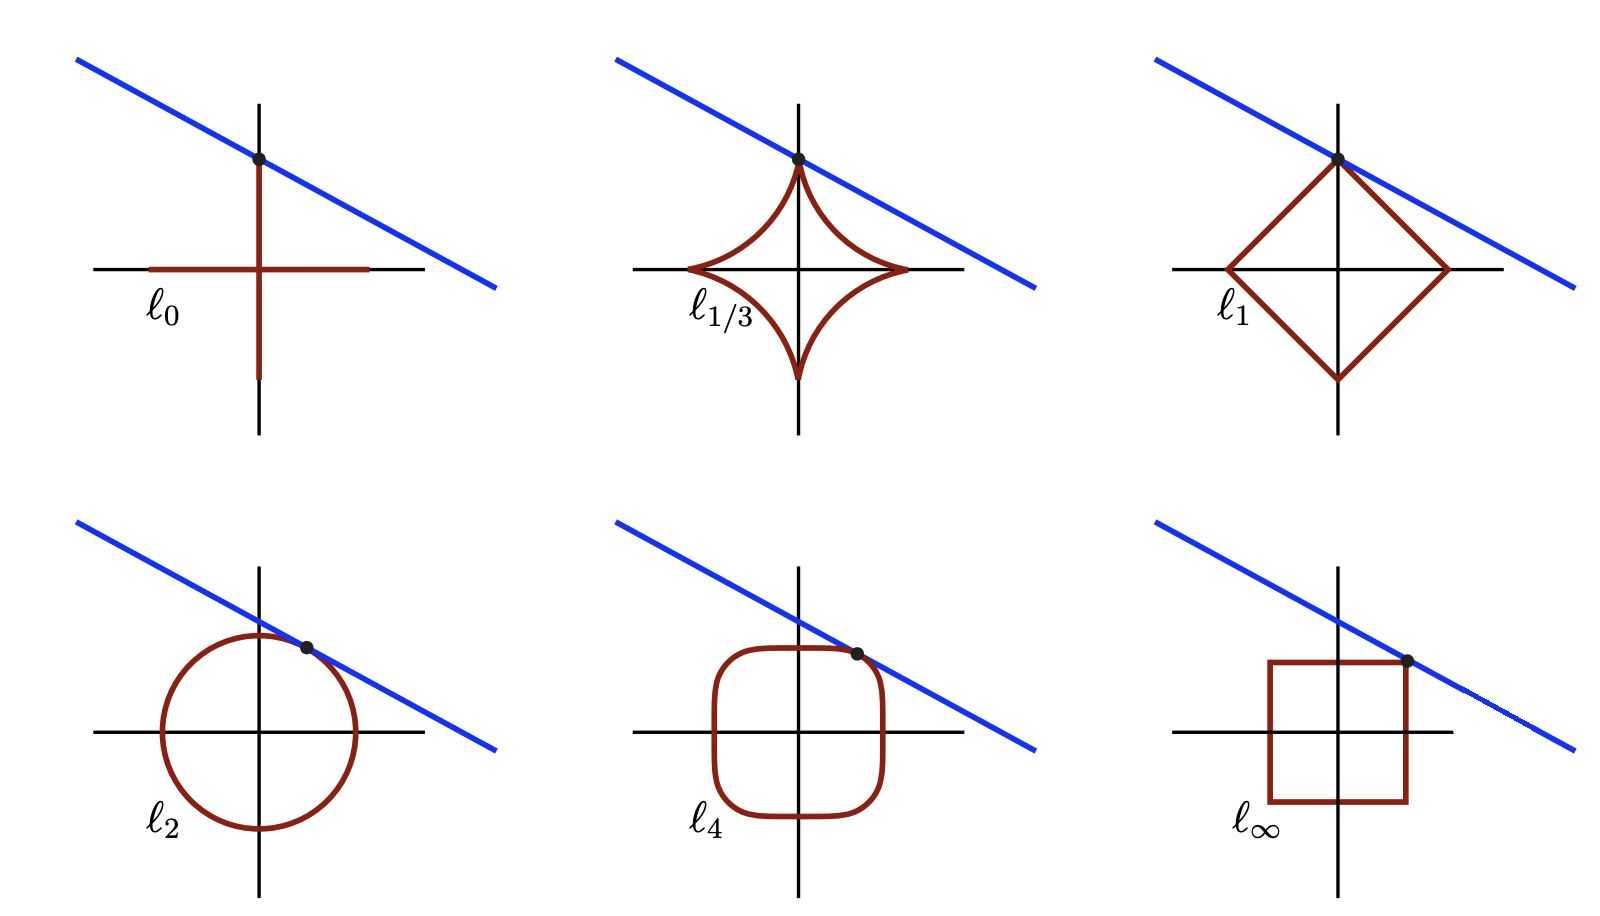
\includegraphics[width=\textwidth]{different_norm.png}
  \caption{不同范数约束项对优化函数的影响}
  \label{fig:different_norm_fig}
\end{figure}

% 在需要插入公式的位置添加以下代码
\begin{equation}
  \begin{aligned}
    \arg\min \Vert \Theta x - y \Vert_2^2 + & \lambda \Vert \Psi a \Vert_0 \\
    \arg\min \Vert \Theta x - y \Vert_2^2 + & \lambda \Vert \Psi a \Vert_1 \\
    \arg\min \Vert \Theta x - y \Vert_2^2 + & \lambda \Vert \Psi a \Vert_2
  \end{aligned}
  \label{eq:different_norm}
\end{equation}

\begin{figure}[ht]
  \centering
  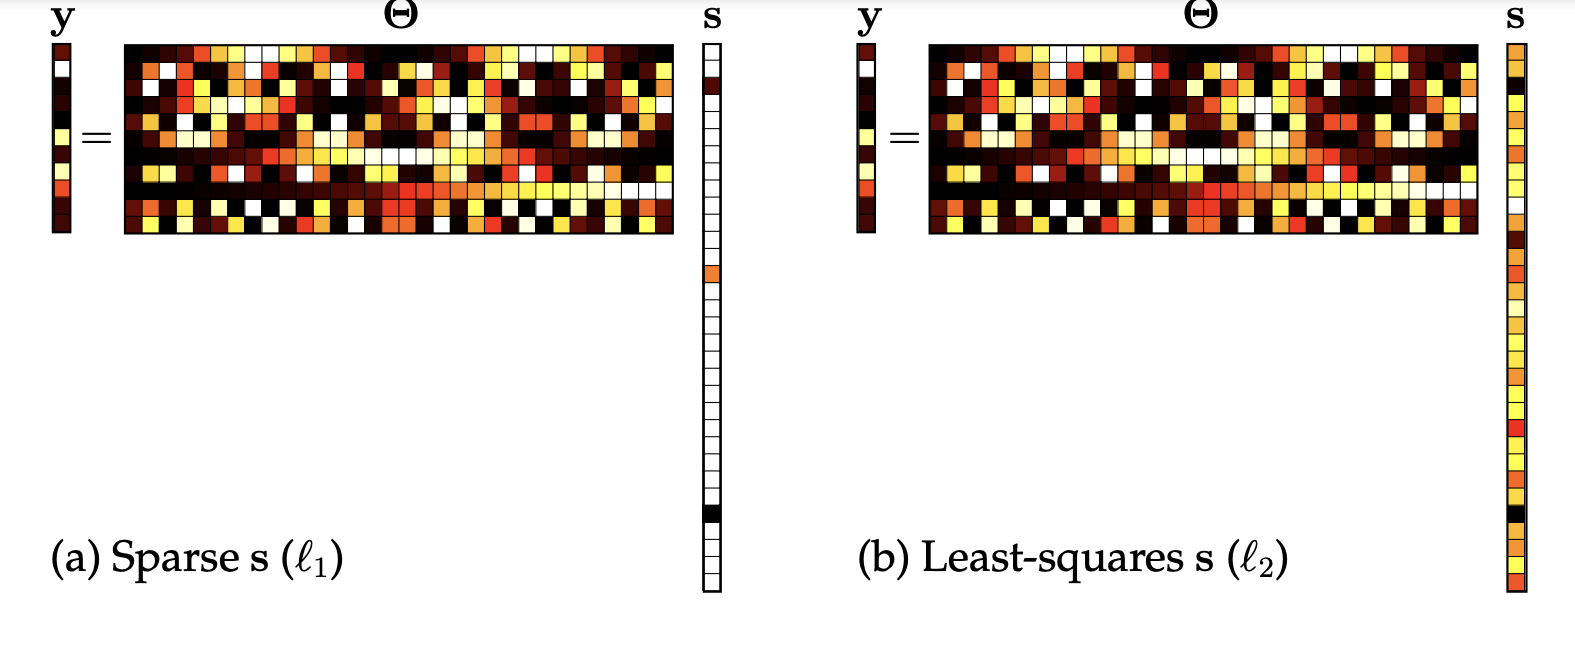
\includegraphics[width=\textwidth]{l1_and_l2_norm.png}
  \caption{l1和l2范数对所得稀疏代码的影响}
  \label{fig:l1_and_l2_norm}
\end{figure}
在上述公式\ref{eq:different_norm}中,$\Vert \Theta x - y \Vert_2^2$是数据保真项,使得最终结果的整体趋势是使得$\Theta x$尽可能地靠近$y$,而后面的$\lambda \Vert \Psi a \Vert_m(m\in N)$作为约束项,为整个公式添加在优化过程中保证稀疏代码的稀疏度的约束。在实践之中,不同范数的约束可形象地表示为图\ref{fig:different_norm_fig}。特别的,针对最常用的l1范数和l2范数约束项,经实验有图\ref{fig:l1_and_l2_norm}结果,表明l2范数约束项在确保稀疏代码稀疏度上效果不如l1。这从图\ref{fig:different_norm_fig}中可以看出,当数据保真项所代表的直线沿着法线方向移动时,l1范数可以确保其在与约束项代表的中央图形接触时,总能够保证唯一的交叉点,根据凸函数性质其即是全局最优点。而在l2范数中,寻找唯一切点的迭代过程是复杂而不确定的,往往会得到两个交点,而无论其中的哪一个都不是最优解。而从范数自身定义考虑,l1范数是稀疏代码所有项绝对值之和,而l2范数是稀疏代码所有项绝对值的开方,后者对于绝对值较大的项相较于前者有放大作用,使得靠近零的项的作用体现较弱,不利于收敛。
